\documentclass[12pt]{amsart}
\usepackage{geometry} % see geometry.pdf on how to lay out the page. There's lots.
\usepackage{graphicx}	% Including figure files
\usepackage{amsmath}	% Advanced maths commands
\usepackage{amssymb}	% Extra maths symbols
\usepackage{hyperref}
\usepackage{float}
\floatplacement{figure}{H}
\floatplacement{table}{H} 
\geometry{a4paper} % or letter or a5paper or ... etc

\title{CSE 546: Machine Learning Homework 3}
\author{David P. Fleming}
\date{November xxx$^{th}$, 2016}

%%% BEGIN DOCUMENT
\begin{document}

\maketitle
\tableofcontents

\section*{Introduction}

Please note that a copy of all the code I wrote to answer the questions in this assignment are included in my submission but also located online at \url{https://github.com/dflemin3/CSE_546/tree/master/HW3}.  Some scripts require data, such as MNIST data, to run to completion and were not included on my github due to file size constraints.  The MNIST data is included in the {\tt Data} directory as python {\tt .pkl} files as this compressed format gave me quicker load times for my scripts.

Overall, my code is structured as follows:  There are three main directories included in my submission: {\tt DML}, {\tt Data} and {\tt HW3}. {\tt HW3} contains all the scripts used to run my analysis.  For example to reproduce the answer for Question 1.2, one would run {\tt python hw3$\_1.2.py$}.  All scripts have relative file paths so the code should run and have detailed comments to describe functionality.  In addition, the scripts have flags near the top to control functionality.  By default, I set all flags to true so the script performs the entire analysis and plotting.  

The {\tt Data} directory contains both the MNIST dataset. The grader should be able to run my homework scripts without altering this directory.  

The {\tt DML} directory contains all the auxiliary files used to do the computations in the homework scripts and has a logical hierarchy.  For example, the directory {\tt optimization} contains the file {\tt gradient$\_$descent.py} while contains both my batch gradient descent and stochastic gradient descent implementations.  The directory {\tt data$\_$processing} contains the script {\tt mnist$\_$utils.py} which contains my functions used to load and work with the MNIST data.  The directory {\tt classification} contains the file {\tt classifier$\_$utils.py} which contains all things related to binary and softmax classification including the gradients for each respective method for use with a gradient descent algorithm.  The {\tt validation} subdirectory contains {\tt validation.py}.  This file contains all my loss functions such as 0/1 loss and also my implementations for regularization paths for both linear regression and logistic and softmax classification using gradient descent.  Finally, the {\tt regression} directory contains all utilities for a normal or multi-class regression.  In particular, this directory contains the file where my ridge regression implementation lives, {\tt ridge$\_$utils.py}. 

In each section, I try to be explicit with what files I used to perform the computation including the path from the {\tt DML} directory for ease of grading.

%%% QUESTION 0  %%%
\section*{Question 0: Collaborators}
I collaborated with Matt Wilde, Serena Liu, and Janet Matsen for various questions on this assignment.

%%% QUESTION 1 %%%

\section*{Question 1: PCA and reconstruction}

TODO

In this question, I solve 10 linear regression problems using regularized Ridge Regression for all 10 digits of the MNIST dataset to build a ``one vs all" classifier.  Each regression is a binary classifier for the corresponding digit.  I classify a sample according to the largest predicted score among my 10 predictors.  The code used to solve this question is in the following attached files: {\tt hw3$\_$1.2.py, hw3$\_$1.3.py, hw3$\_$1.4.py} in the {\tt HW3} directory and {\tt classification/classifier$\_$utils.py, regression/regression$\_$utils.py, validation/validation.py, data$\_$processing/mnist$\_$utils.py} in the {\tt DML} directory.

\subsection*{1.1: Matrix Algebra Review}

TODO

\subsection*{1.2: PCA}

\subsubsection*{1.2.1}

TODO

\subsubsection*{1.2.2}

TODO

\begin{figure}[H]
	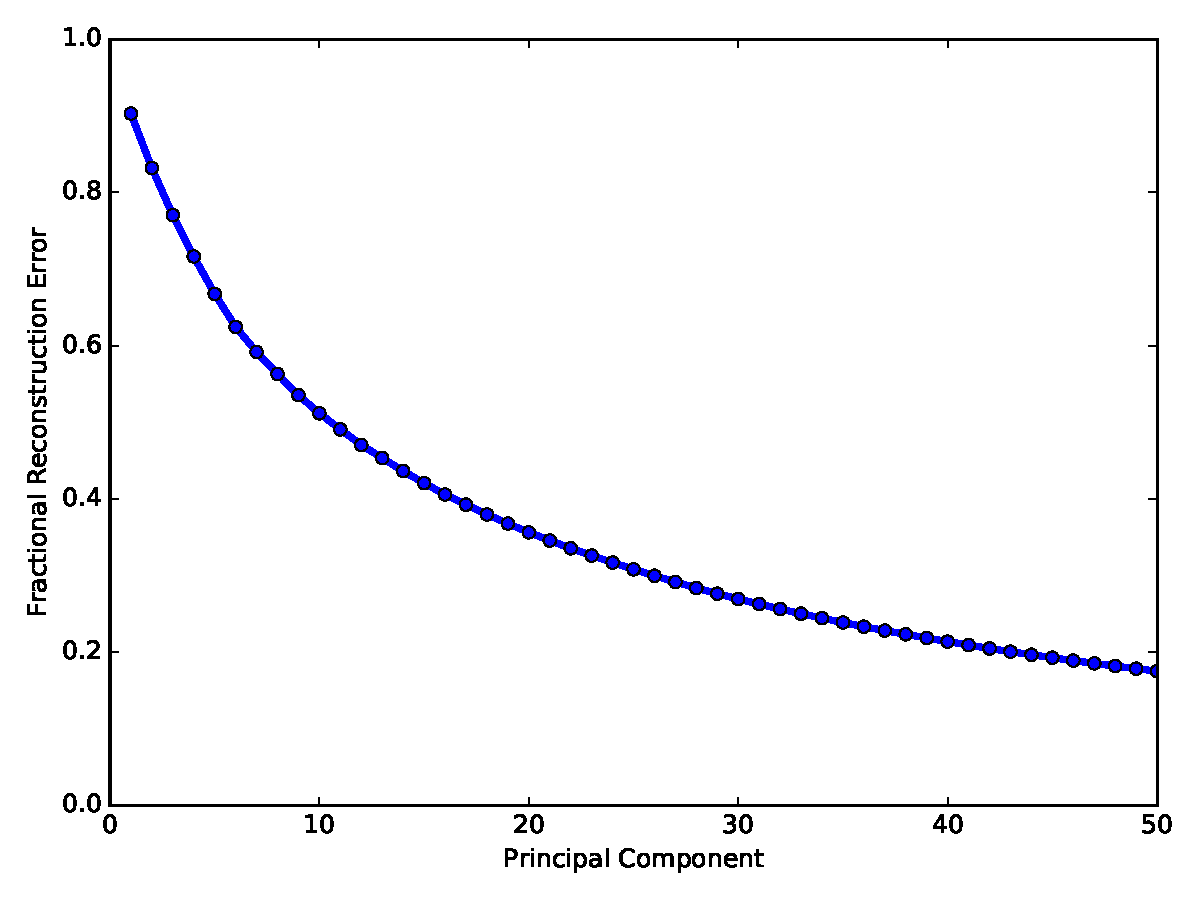
\includegraphics[width=\columnwidth]{fractional_rec_error.pdf}
    \caption{Fractional reconstruction error as a function of $k$ principal components out of $d$ total dimensions for $k \in [1,50]$.}
    \label{fig:frac_rec_error}
\end{figure}


\subsubsection*{1.2.3}

TODO

\subsubsection*{1.2.4}

TODO

\begin{figure}[H]
	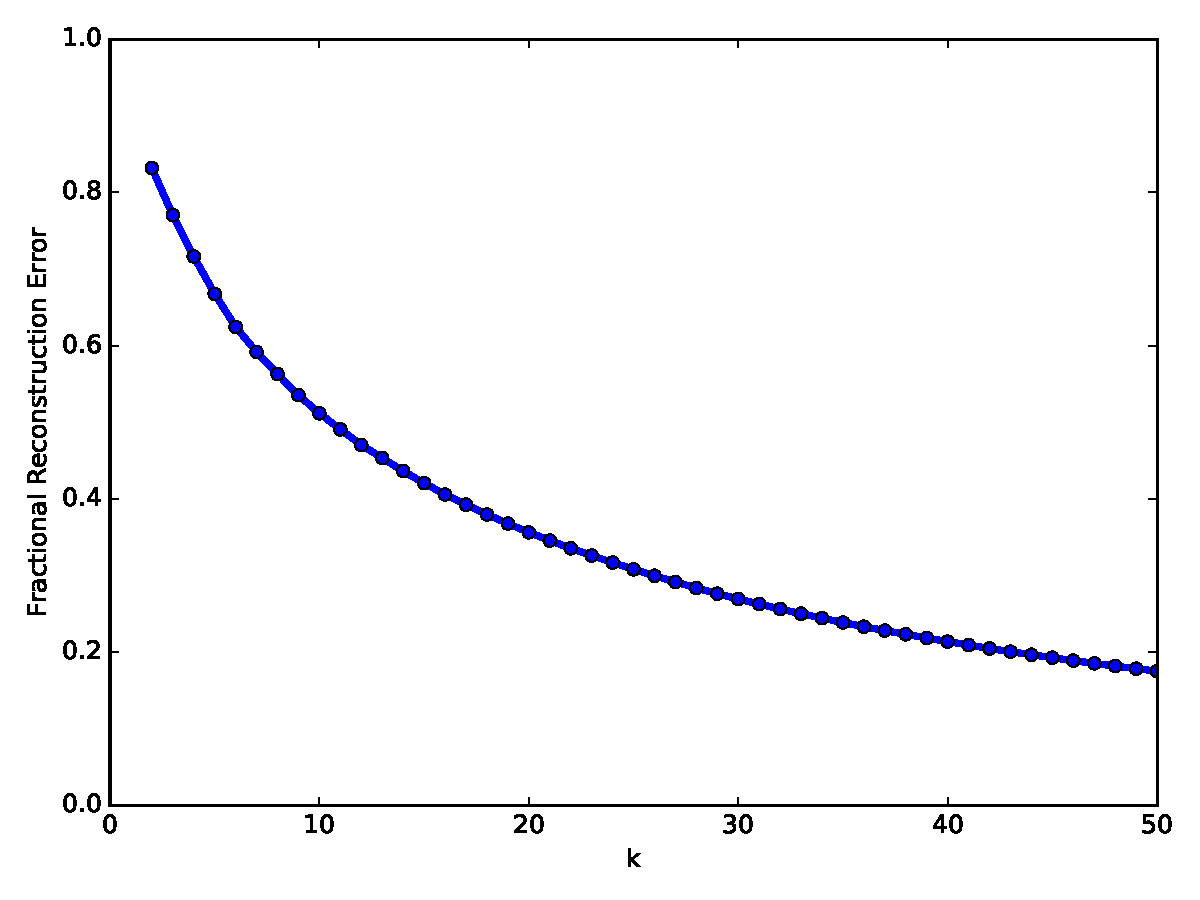
\includegraphics[width=\columnwidth]{fractional_rec_error_sans_mean.pdf}
    \caption{Fractional reconstruction error as a function of $k$ principal components out of $d$ total dimensions for $k \in [2,50]$.}
    \label{fig:frac_rec_error_sans_mean}
\end{figure}

\subsection*{1.3: Visualization of the Eigen-Directions}

\subsubsection*{1.3.1}

TODO

\begin{figure}[H]
	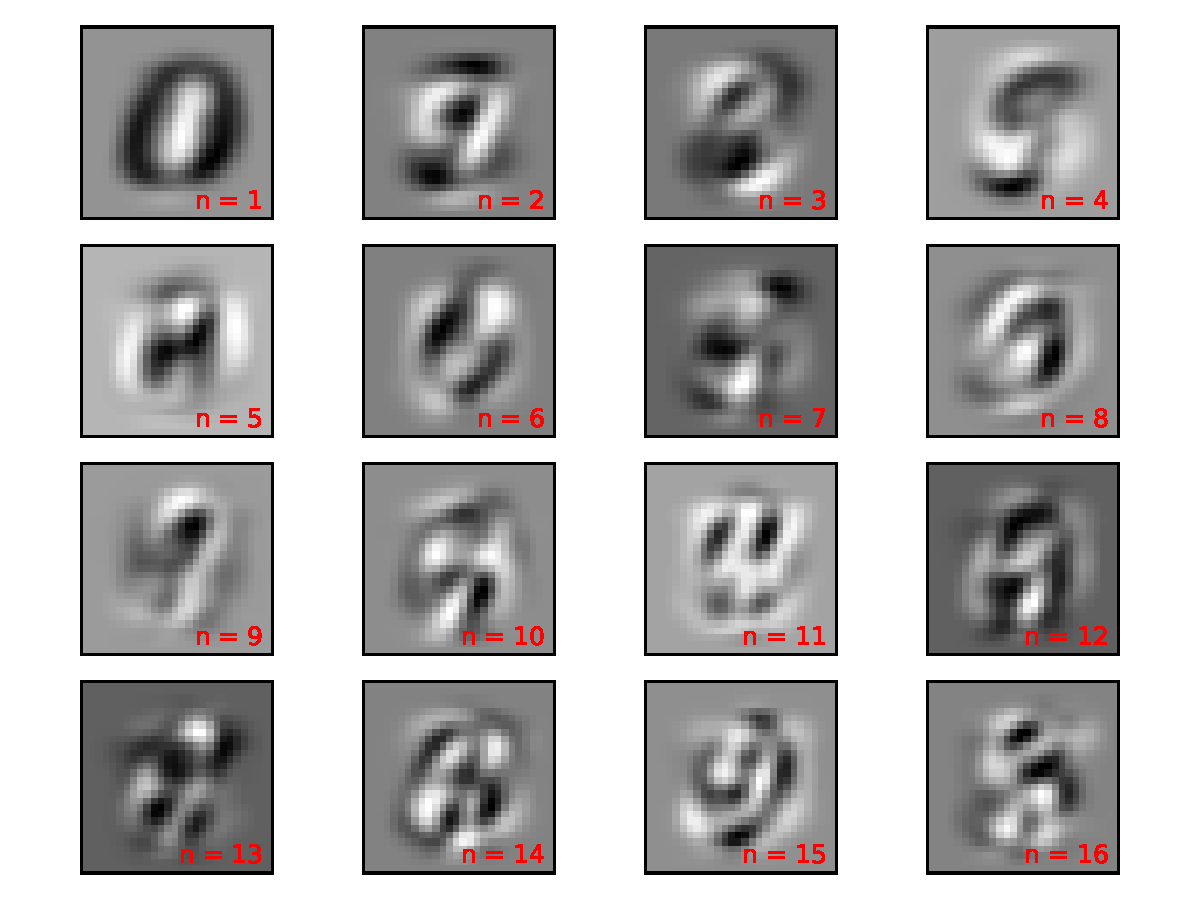
\includegraphics[width=\columnwidth]{eigendirections.pdf}
    \caption{Visualization of the first 16 eigendirections as $28 \times 28$ pixel images.  The respective eigendirection number is given in red in a subplot's lower righthand corner.}
    \label{fig:eigendirections}
\end{figure}

\subsubsection*{1.3.2}

TODO: eigen-interpretations

\subsection*{1.4: Visualization and Reconstruction}

TODO

\subsubsection*{1.4.1}

\begin{figure}[H]
	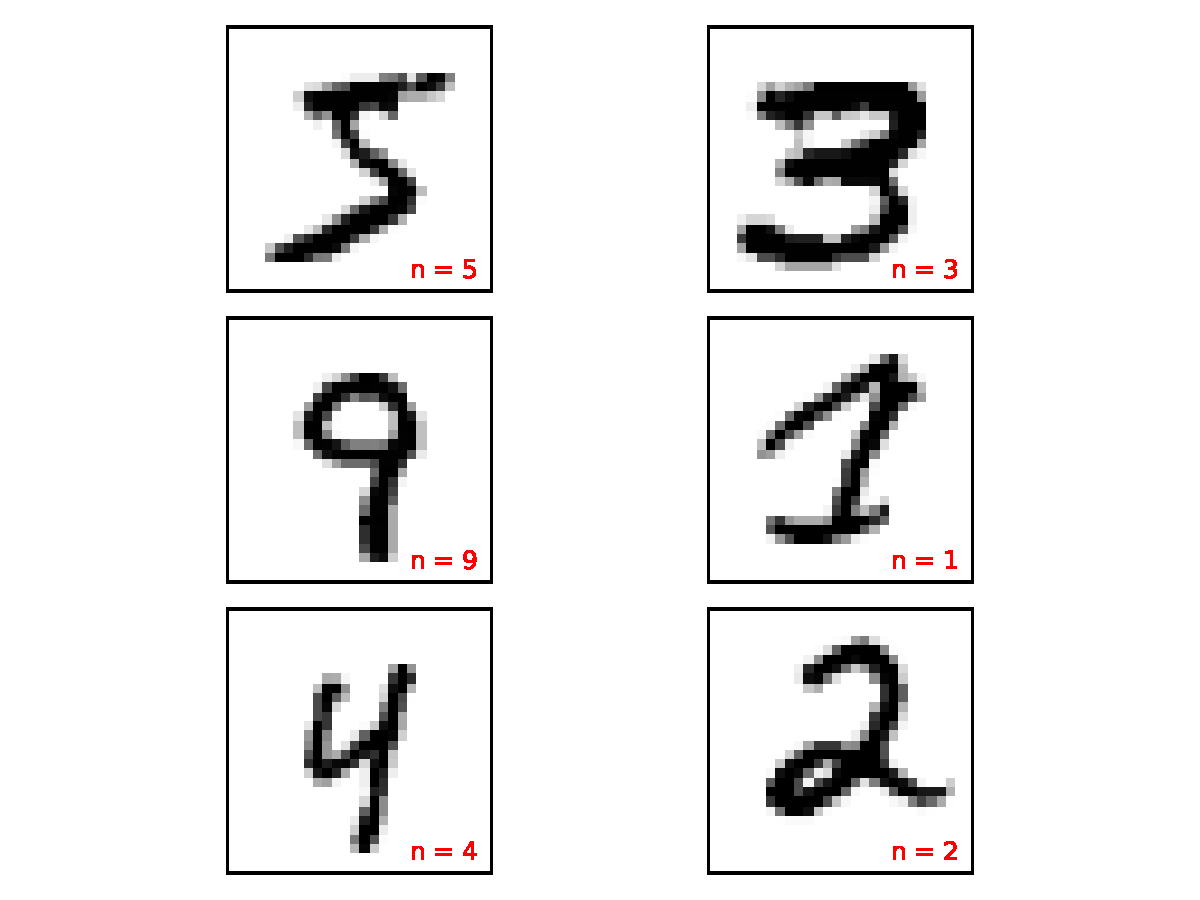
\includegraphics[width=\columnwidth]{mnist_digits.pdf}
    \caption{Visualization of 6 random, unique digits from the MNIST training set.  The image label is displayed in red in the lower-righthand corner of each image.}
    \label{fig:mnist_digits}
\end{figure}

\subsubsection*{1.4.2}

\begin{figure}[H]
	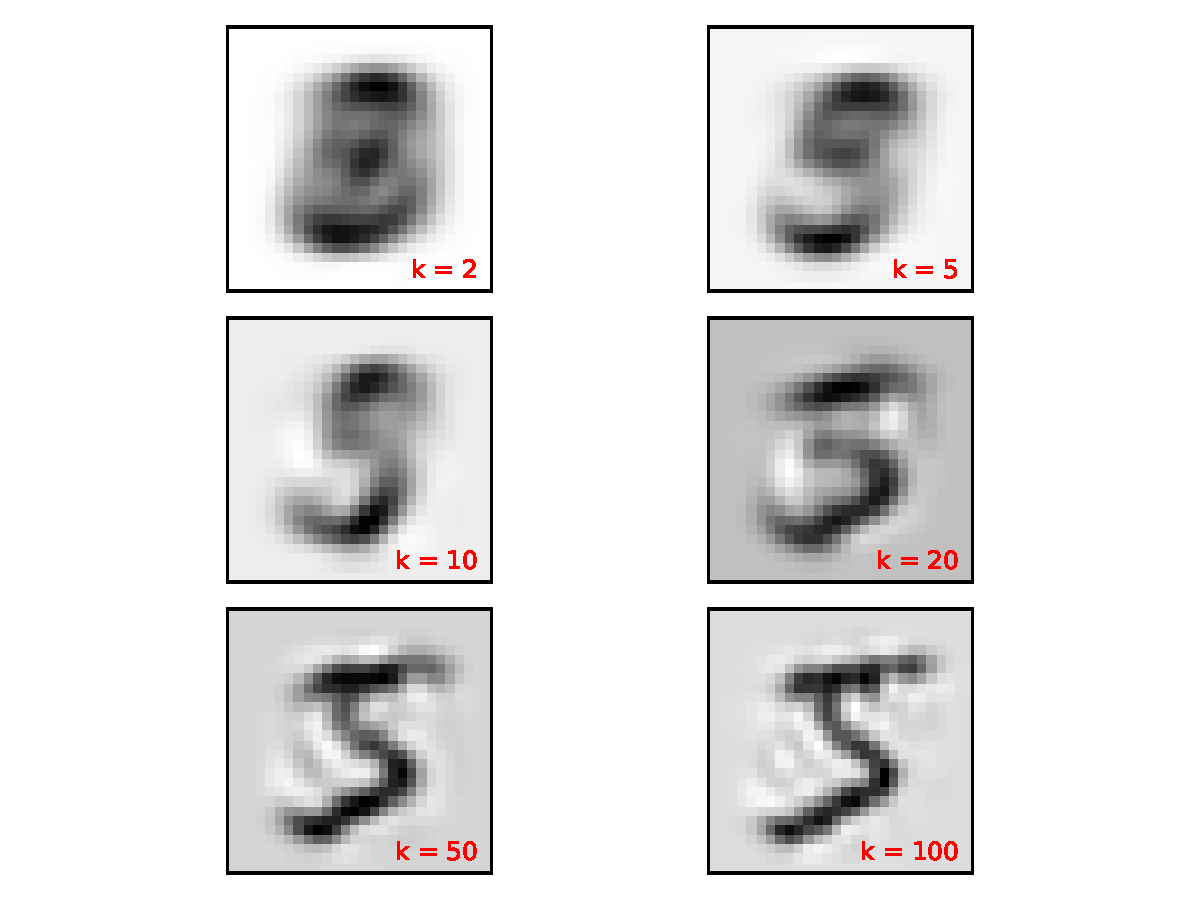
\includegraphics[width=\columnwidth]{5_recon_mnist.pdf}
    \caption{Reconstruction of a number 5 from the MNIST data set (see Fig.~\ref{fig:mnist_digits} using $k \in [2,5,10,20,50,100]$ principal components where the given $k$ is denoted in red in the lower-righthand corner of the respective subplot.}
    \label{fig:recon_5}
\end{figure}

\begin{figure}[H]
	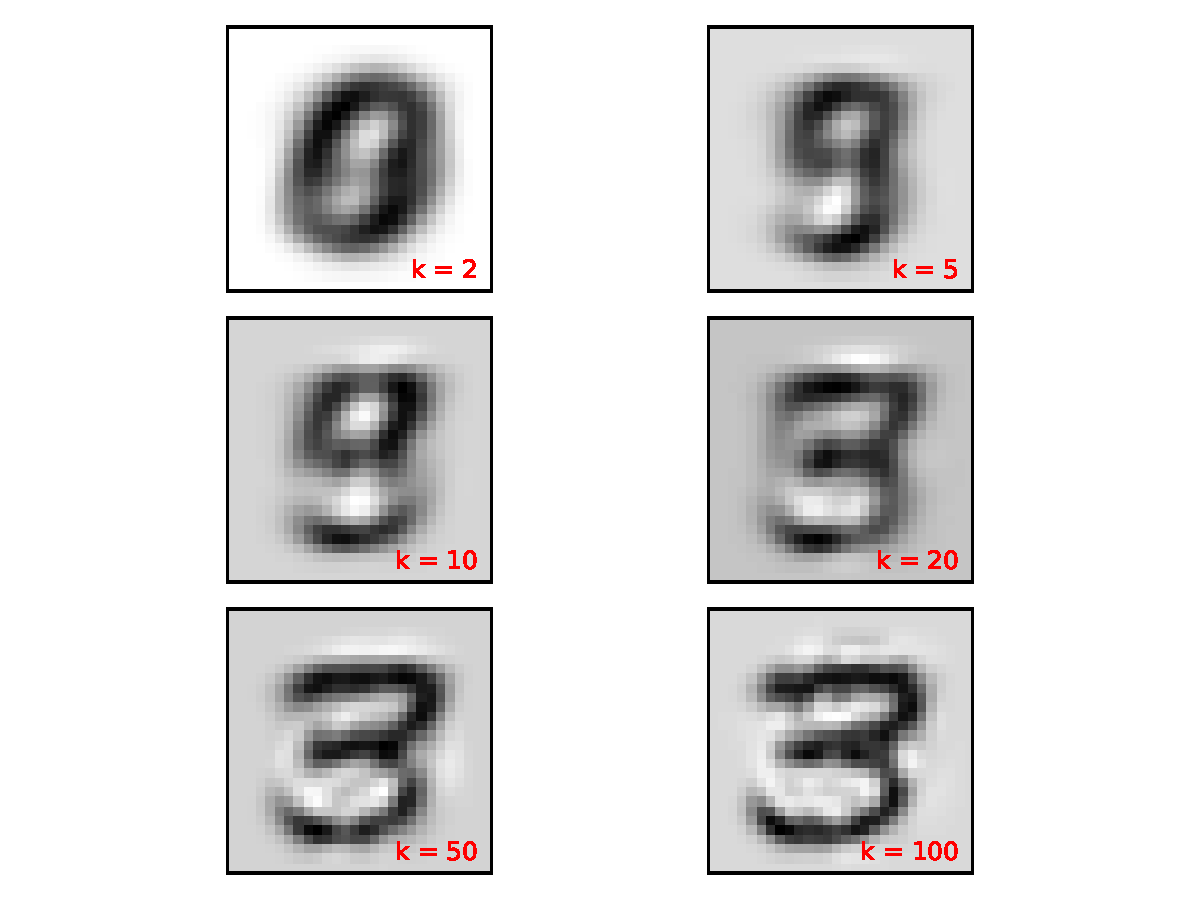
\includegraphics[width=\columnwidth]{3_recon_mnist.pdf}
    \caption{Reconstruction of a number 3 from the MNIST data set (see Fig.~\ref{fig:mnist_digits}) using $k \in [2,5,10,20,50,100]$ principal components where the given $k$ is denoted in red in the lower-righthand corner of the respective subplot.}
    \label{fig:recon_3}
\end{figure}

\begin{figure}[H]
	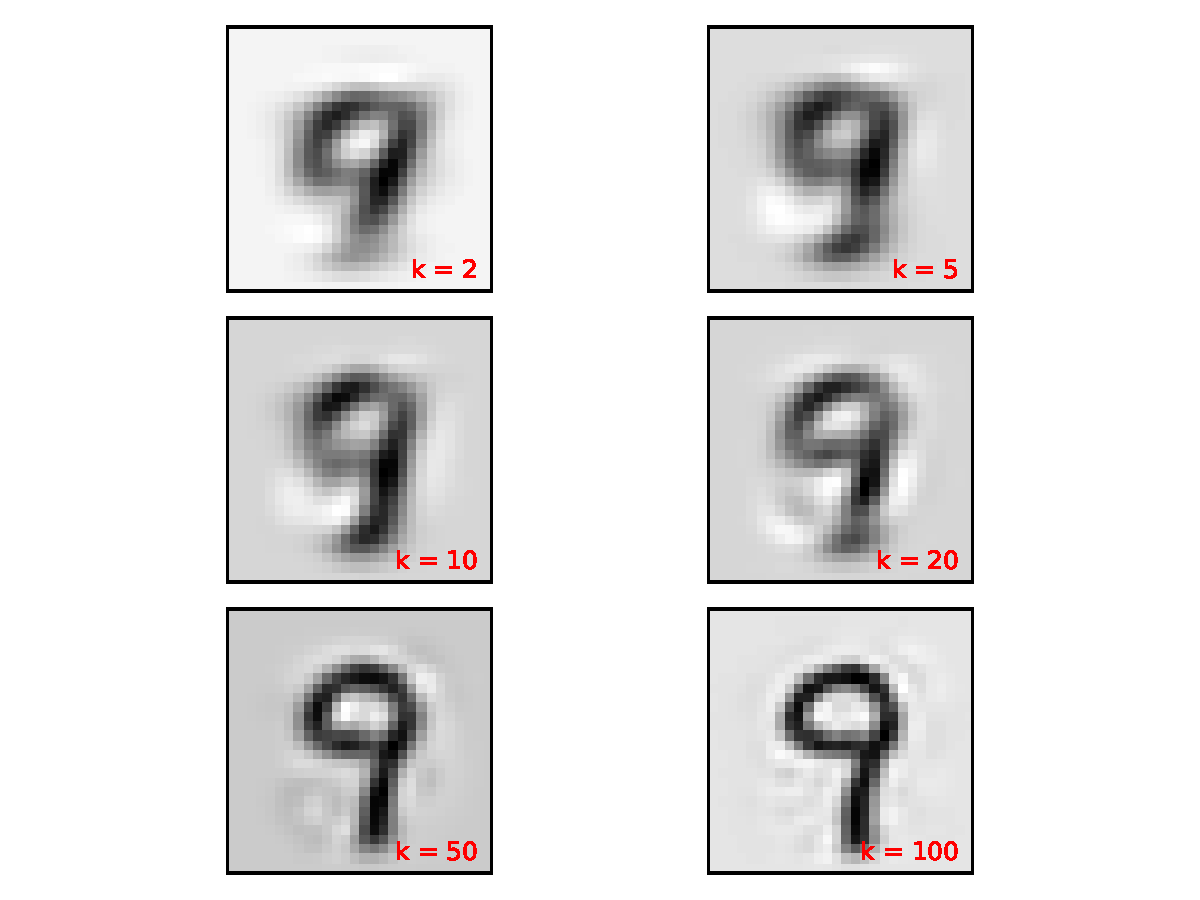
\includegraphics[width=\columnwidth]{9_recon_mnist.pdf}
    \caption{Reconstruction of a number 9 from the MNIST data set (see Fig.~\ref{fig:mnist_digits}) using $k \in [2,5,10,20,50,100]$ principal components where the given $k$ is denoted in red in the lower-righthand corner of the respective subplot.}
    \label{fig:recon_9}
\end{figure}

\begin{figure}[H]
	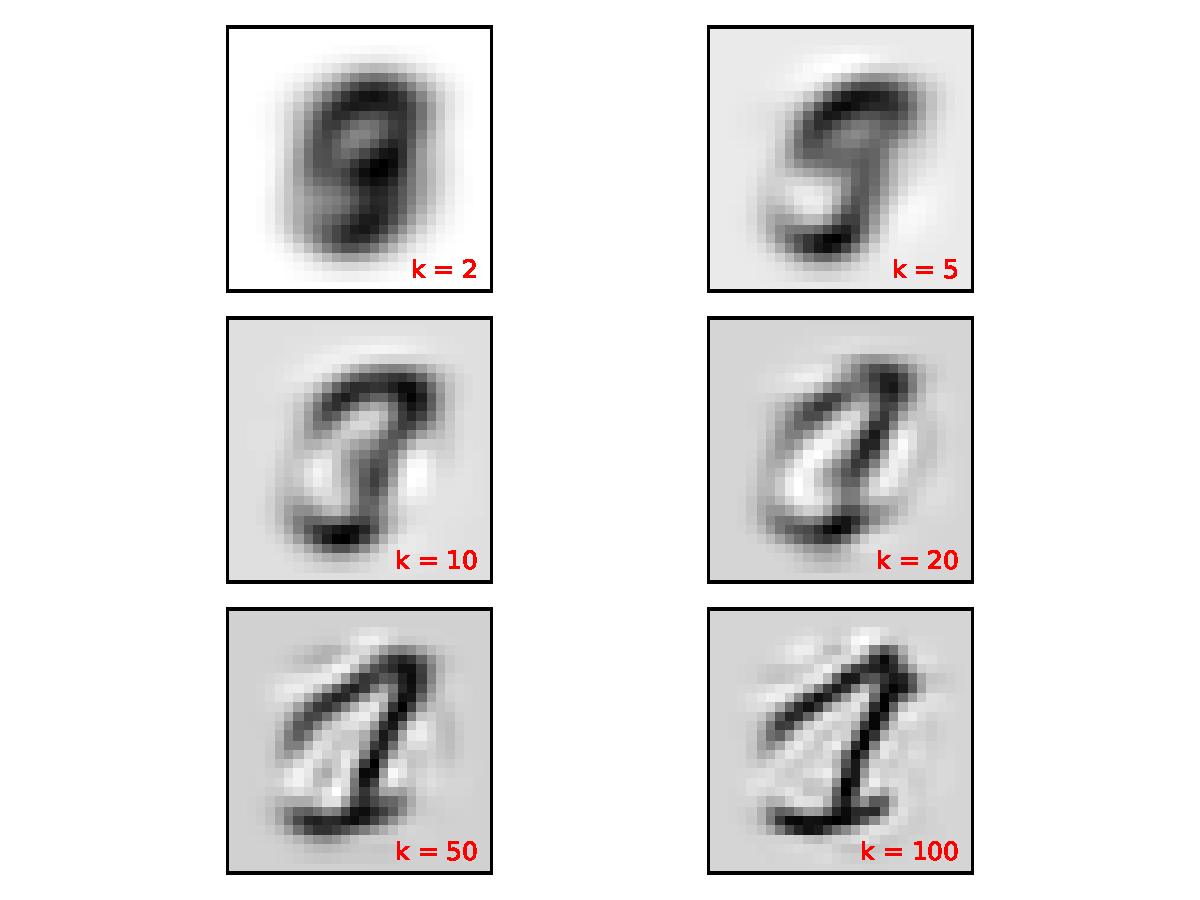
\includegraphics[width=\columnwidth]{1_recon_mnist.pdf}
    \caption{Reconstruction of a number 1 from the MNIST data set (see Fig.~\ref{fig:mnist_digits}) using $k \in [2,5,10,20,50,100]$ principal components where the given $k$ is denoted in red in the lower-righthand corner of the respective subplot.}
    \label{fig:recon_1}
\end{figure}

\begin{figure}[H]
	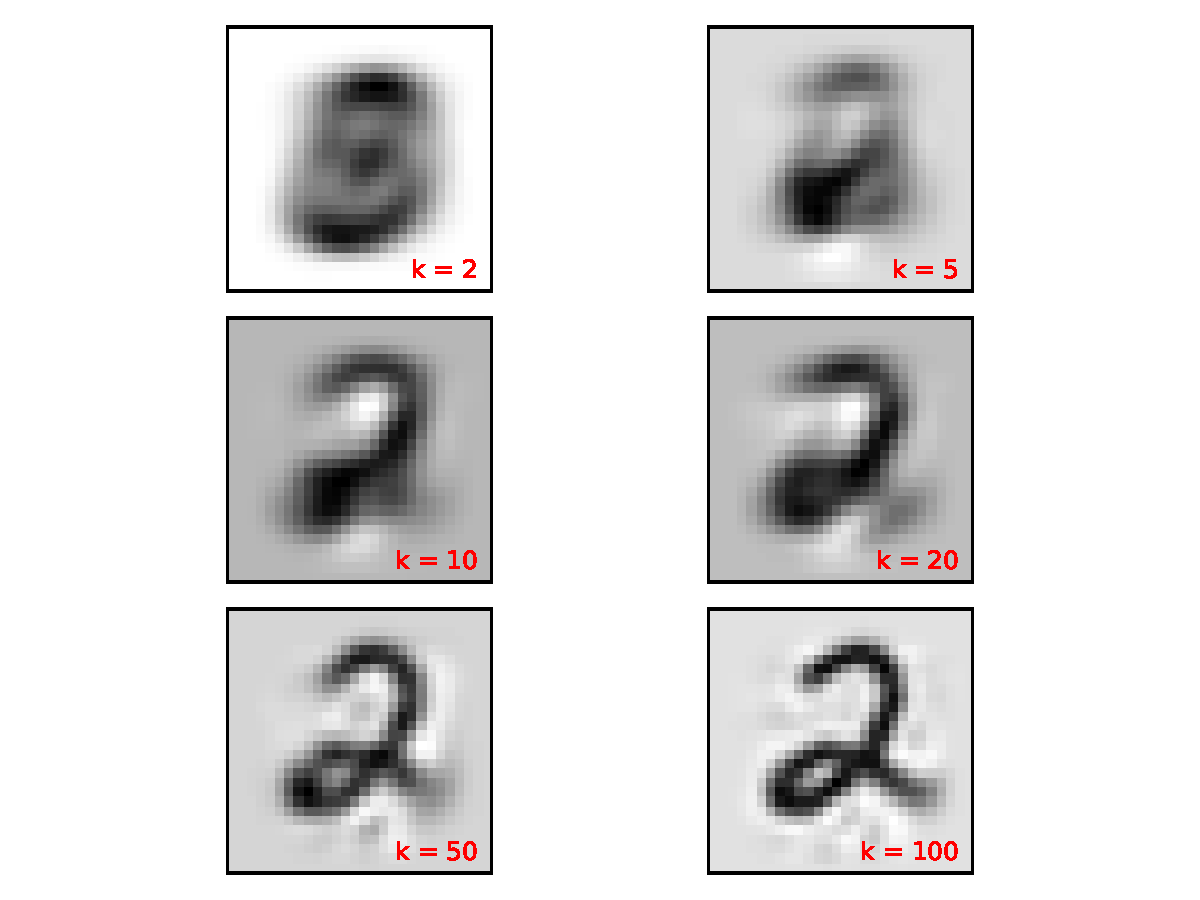
\includegraphics[width=\columnwidth]{2_recon_mnist.pdf}
    \caption{Reconstruction of a number 2 from the MNIST data set (see Fig.~\ref{fig:mnist_digits}) using $k \in [2,5,10,20,50,100]$ principal components where the given $k$ is denoted in red in the lower-righthand corner of the respective subplot.}
    \label{fig:recon_2}
\end{figure}

\begin{figure}[H]
	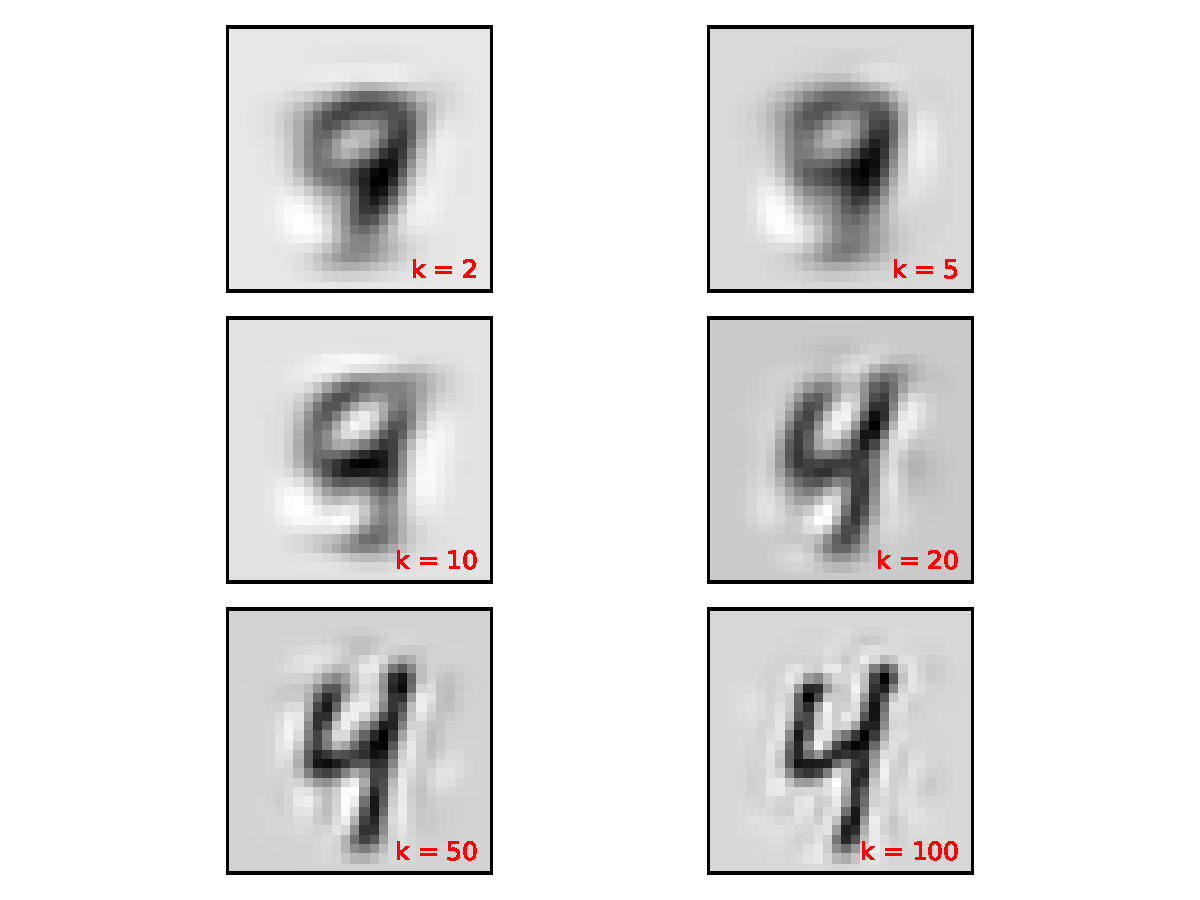
\includegraphics[width=\columnwidth]{4_recon_mnist.pdf}
    \caption{Reconstruction of a number 4 from the MNIST data set (see Fig.~\ref{fig:mnist_digits}) using $k \in [2,5,10,20,50,100]$ principal components where the given $k$ is denoted in red in the lower-righthand corner of the respective subplot.}
    \label{fig:recon_4}
\end{figure}

\subsubsection*{1.4.3}

TODO



\end{document}